%=============================--A--=============================%
\newpage
\section{Introdução}
Na multiplexaç\~ao estereofónica, transmitem-se 2 mensagens em simultâneo utilizando a mesma portadora: uma associada ao ouvido direito, $R$, e a outra ao esquerdo, $L$.

A mensagem enviada num sinal stereo é da forma:

\begin{equation*}
    m(t)=\underbrace{\overbrace{[L+R]}^{\text{$m_1(t)$}}}_{\substack{\text{Componente}\\ \text{monofónica}}}+\ \underbrace{\overbrace{[L-R]}^{m_2(t)}\cdot\cos{(4\pi f_c t)}}_{\substack{\text{Componente estereofónica}\\ \text{DSB-SC}}} + \underbrace{K\cdot\cos{(2\pi f_c t)}}_{\text{Subportadora piloto}}
\end{equation*}

A {\hyperref[fig:stereo_spectrum]{Fig. 1}} explícita o formato espectral da mensagem, em que a banda dos sinais $m_1(t)$ e $m_2(t)$ é $B=15$ kHz e a frequência da subportadora é $f_c=19$ kHz (relevante mais tarde na parametrizaç\~ao dos filtros do processo de descodificaç\~ao).
%portadora auxiliar??
%desprezar o de 57k e de 67k (nota de rodapé?) boa ideia

\begin{figure}[H]
    \centering
    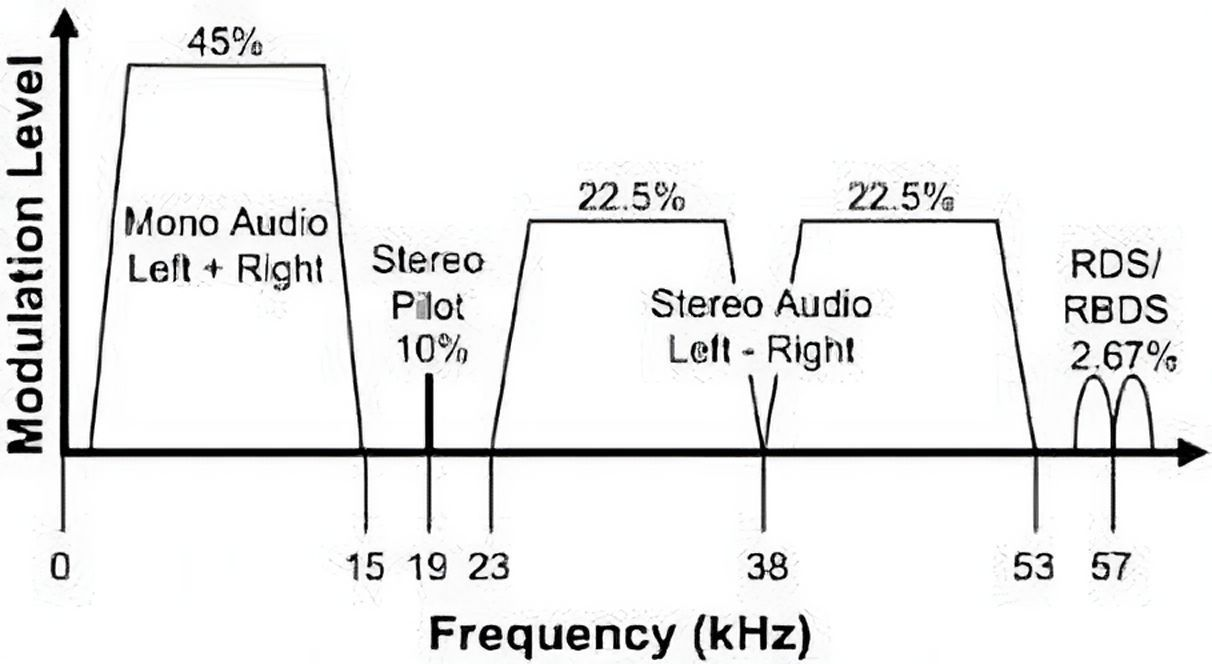
\includegraphics[width = 0.6\linewidth]{img/mpx_signal_spectrum.jpeg}
    \caption{Espectro da mensagem de um sinal FM stereo.}
    \label{fig:stereo_spectrum}
\end{figure}

Após a recuperaç\~ao dos sinais $m_1(t)$ e $m_2(t)$, obtém-se trivialmente os sinais desejados, $L$ e $R$, através do processo de \textit{dematrixing}:

\begin{equation*}
  \left\{\begin{array}{@{}l@{}}
    m_1(t)+m_2(t)=2L\\
    m_1(t)-m_2(t)=2R
  \end{array}\right.\,.
\end{equation*}

Apresenta-se então, na \hyperref[fig:desmodulador FM stereo]{Fig. 2} um esquema simplificado do processo de desmultiplexaç\~ao, posterior à desmodulaç\~ao do sinal FM.

\begin{figure}[H]
    \centering
    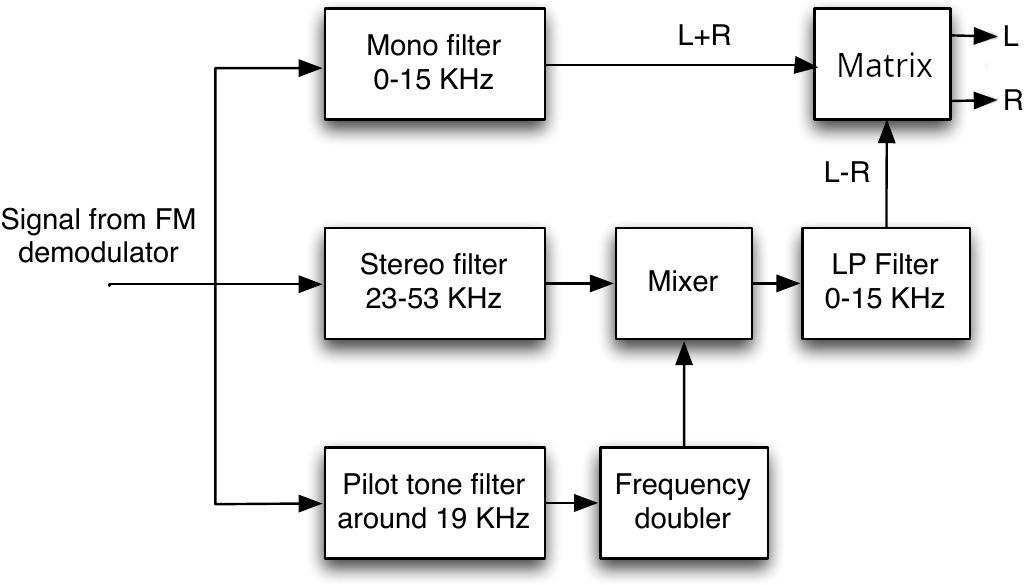
\includegraphics[width = 0.6\linewidth]{img/stereo_demultiplexing.jpeg}
    \caption{Modelo simplificado do descodificador stereo.}
    \label{fig:desmodulador FM stereo}
\end{figure}
%1
%1
%=============================--B--=============================%
\newpage
\subsection{Desmodulaç\~ao de um sinal FM}
Na secção anterior partimos do princípio que já temos o sinal m(t), mas na transmiss\~ao de um sinal FM é realizado uma modulação da mensagem, tal que o sinal que o recetor recebe é o seguinte:

\begin{equation*}
    x_{FM}(t)=A_c \cos{(2\pi f_c t + 2 \pi k_f  \int_{-\infty}^{t} m(\lambda) \,d\lambda)}
\end{equation*}

É então nossa tarefa recuperar a mensagem m(t) a partir do sinal $x_{FM}(t)$. Para tal existem 2 opções:

\vspace{0.5em}
\textbf{Opção 1:}
Uma vez que a mensagem está na frequência do cosseno, a opção mais intuitiva seria derivar o sinal $x_{FM}(t)$ e utilizar um detetor de envolvente.

\begin{equation*}
    \frac{1}{2\pi} \frac{\partial x_{FM}(t)}{\partial x} =
    A_c (f_c + k_f m(t))\cos{\left(2\pi f_c t + 2 \pi k_f  \int_{-\infty}^{t} m(\lambda) \,d\lambda + \frac{\pi}{2}\right)}
\end{equation*}

Uma vez que a amplitude do sinal resultante segue o andamento de m(t), pode-se utilizar um detetor de envolvente para recuperar a mensagem.

\vspace{1.5em}

\textbf{Opção 2:}

Utilizar um desmodulador em quadratura. 
Este desmodulador começa com um misturador que faz a heterodinagem do sinal, "arrastando-o" de modo a ficar centrado em $f_I$ em vez de $f_c$, visto que os filtros posteriores estão centrados nessa frequência.

De seguida através do produto por um cosseno e um sinal retira a componente em fase ($x_I(t)$) e em quadratura ($x_Q(t)$) do sinal $x_{FM}(t)$. Obtendo-se o seguinte sinal:

\begin{equation*}
    x(t)=x_I(t)\cos{(2 \pi f_I t)} - x_Q(t)\sin{(2 \pi f_I t)}
\end{equation*}

em que:

\begin{equation*}
  \left\{\begin{array}{@{}l@{}}
    x_I(t)= A_x \cos{(2 \pi k_f  \int_{-\infty}^{t} m(\lambda) \,d\lambda)}\\
    x_Q(t)= A_x \sin{(2 \pi k_f  \int_{-\infty}^{t} m(\lambda) \,d\lambda)}
  \end{array}\right.\,.
\end{equation*}

A partir das componentes em fase e quadratura, é simples descobrir a mensagem, uma vez que:

\begin{equation*}
    \frac{1}{2\pi} \arctan{\left(\frac{x_Q(t)}{x_I(t)}\right)}= k_f  \int_{-\infty}^{t} m(\lambda) \,d\lambda
\end{equation*}

Derivando o $\arctan{}$ e organizando as parcelas, obtém-se que a mensagem é dada por:

\begin{equation*}
    \therefore m(t) = \frac{1}{2\pi k_f} \frac{\partial}{\partial x}\left[\arctan{\left(\frac{x_Q(t)}{x_I(t)}\right)}\right]
\end{equation*}
